\section{Space Discretization} \todo{Begynn på nytt på dette..}
For the two-dimensional case, we rewrite the right hand side of \eqref{eq:model1-pde} in order to see if it can be simplified. 

\begin{proposition}\label{prop:simplification-equation}
In two spatial dimensions, \eqref{eq:pde-eq1-num} can be written as
\begin{equation}
    u_t = (1-\alpha)\, \frac{u_x^2 u_{yy} - 2 u_{xy} u_x u_y + u_y^2u_{xx}}{u_x^2 + u_y^2} + (u_x^2 + u_y^2)^{\frac{1}{2}}\alpha \sigma d
    \label{eq:pde-written-out}
\end{equation}
\end{proposition}

\begin{proof}
\begin{equation}\label{eq:proof-writeout}
    \begin{aligned}
        u_t &= |\nabla u| \bigg[(1-\alpha)\,(\nabla \cdot \bigg(\frac{\nabla u}{|\nabla u|}\bigg) + \alpha d \bigg] \\ &= |\nabla u|\,(1-\alpha)\,\bigg( \nabla \cdot \bigg(\frac{\nabla u}{|\nabla u|}\bigg) \bigg) + |\nabla u| \alpha d
    \end{aligned}
\end{equation}
The last term can not be simplified further, so we will only look further into the first term.

Using the product rule, we get
\begin{equation*}
    \nabla \cdot \bigg(\frac{\nabla u}{|\nabla u|}\bigg) = \frac{\Delta u}{|\nabla u|} + \nabla u \cdot \nabla\bigg( \frac{1}{|\nabla u|}\bigg)
\end{equation*}

Writing out the gradient operators for each term, we obtain
\begin{align}
    |\nabla u| &= (u_x^2+u_y^2)^{\frac{1}{2}} \label{eqs:grads-1}\\
    \Delta u &= (u_{xx} + u_{yy}) \label{eqs:grads-2}\\
    \nabla u &= \begin{bmatrix}u_x & u_y \end{bmatrix} \label{eqs:grads-3}\\
    \nabla \bigg( \frac{1}{|\nabla u|} \bigg) &= \begin{bmatrix}\bigg( \frac{1}{|\nabla u|} \bigg)_x & \bigg( \frac{1}{|\nabla u|} \bigg)_y \end{bmatrix} \label{eqs:grads-4}\\
    \bigg( \frac{1}{|\nabla u|} \bigg)_x &= -\frac{1}{2} (u_x^2+u_y^2)^{-\frac{3}{2}}(2u_x u_{xx}+2u_y u_{xy}) \label{eqs:grads-5}\\
    \bigg( \frac{1}{|\nabla u|} \bigg)_y &= -\frac{1}{2} (u_x^2+u_y^2)^{-\frac{3}{2}}(2u_y u_{yy}+2u_x u_{xy}) \label{eqs:grads-6}
\end{align}

Using \eqref{eqs:grads-1}-\eqref{eqs:grads-6}, we obtain
\begin{equation*}
    \begin{gathered}
        |\nabla u|\, \bigg(\nabla \cdot \bigg(\frac{\nabla u}{|\nabla u|}\bigg)\bigg)
        = (u_x ^2 + u_y ^2)^{\frac{1}{2}} \bigg( \frac{\Delta u}{|\nabla u|} + \nabla u \cdot \nabla \bigg(\frac{1}{|\nabla u|} \bigg) \bigg) \\
        = (u_x ^2 + u_y ^2)^{\frac{1}{2}} \bigg[ (u_{xx} + u_{yy}) (u_x ^2 + u_y ^2)^{-\frac{1}{2}} - \frac{1}{2} (u_x ^2 + u_y ^2)^{-\frac{3}{2}} (2u_x^2u_{xx}+4u_x u_{xy} u_y + 2u_y^2 u_{yy})\bigg] \\
        = (u_{xx} + u_{yy}) - \frac{1}{u_x^2+u_y^2} (u_x^2 u_{xx}+2u_{xy} u_x u_y + u_y^2 u_{yy}) \\
        = \frac{1}{u_x^2+u_y^2} ( (u_{xx} + u_{yy})(u_x^2 + u_y^2) - u_x^2 u_{xx}-2u_{xy} u_x u_y - u_y^2 u_{yy}) \\
        = \frac{1}{u_x^2+u_y^2}(u_{xx}u_x^2 + u_{yy}u_x^2 + u_y^2u_{xx}+ u_y u_{yy}-u_x^2 u_{xx}-2u_{xy} u_x u_y - u_y^2 u_{yy}) \\
        = \frac{u_x^2u_{yy} - 2u_{xy}u_xu_y + u_y^2u_{xx}}{u_x^2+u_y^2}.
    \end{gathered}
\end{equation*}

Thus 
\begin{equation*}
    u_t =(1-\alpha)\, \frac{u_x^2 u_{yy} - 2 u_{xy} u_x u_y + u_y^2u_{xx}}{u_x^2 + u_y^2} + (u_x^2 + u_y^2)^{\frac{1}{2}}\alpha d
\end{equation*}
\end{proof}

This means that 

\subsection*{A Finite Difference Scheme}
We want to implement a finite difference approximation on our domain $\mathcal{D} = [x_{\text{start}}, x_{\text{end}}]\times[y_{\text{start}}, y_{\text{end}}]$. To make a uniform discretization of the domain, \domain, we divide the $x-$ and $y-$axis with respectively $N_x$ vertical lines and $N_y$ horizontal lines equally distributed. In every crossing of such lines, there are nodal points, which gives a total of $N_x\times N_y$ nodal points in our domain. Since the grid is uniform, the horizontal distance between the nodal points will be $\Delta x = \frac{x_{\text{end}} - x_{\text{start}}}{N_x-1}$ and $\Delta y = \frac{y_{\text{end}} - y_{\text{start}}}{N_y-1}$ in vertical direction. 

We then denote the nodal points with coordinates $[x_i, y_j] = [x_0 + i\Delta x, y_0+j\Delta y]$ where $x_0 = x_{\text{start}}$ and $y_0 = y_{\text{start}}$. The value of our function \uxt at the nodal point $[x_i, y_j]$  at a certain time $t_n$ is then denoted $U_{i, j}|^n = u(x_i, y_i; t_n)$. These are the approximated values of our function. In addition, to be able to approximate the time derivative $u_t$ from \eqref{eq:model1-pde}, we need the discretized curvature and gradient of our function \uxt. We begin with listing the standard central difference approximations for the first and second order derivatives in addition the the mixed derivative.

\begin{align}
    u_x (x_i, y_j) &= \frac{\Uipj - \Uinj}{2\Delta x} \label{eq:x-deriv}\\
    u_y (x_i, y_j) &= \frac{\Uijp - \Uijn}{2\Delta y} \label{eq:y-deriv} \\
    u_{xx} (x_i, y_j) &= \frac{\Uipj-2\Uij+\Uinj}{\Delta x ^2} \label{eq:x-doublederiv} \\
    u_{yy} (x_i, y_j) &= \frac{\Uijp - 2\Uij + \Uijn}{\Delta y^2} \label{eq:y-doublederiv} \\
    u_{x, y} (x_i, y_j) &= \frac{\Uipjp-\Uipjn-\Uinjp+\Uinjn}{4\Delta x \Delta y}
\end{align}

Looking at \eqref{eq:pde-written-out} we see that the resulting stencil for inserting the discretized operators into \eqref{eq:pde-written-out} will be a eight-pointed star as shown in \figref{fig:stencil+grid}.


\begin{figure}
    \centering
    

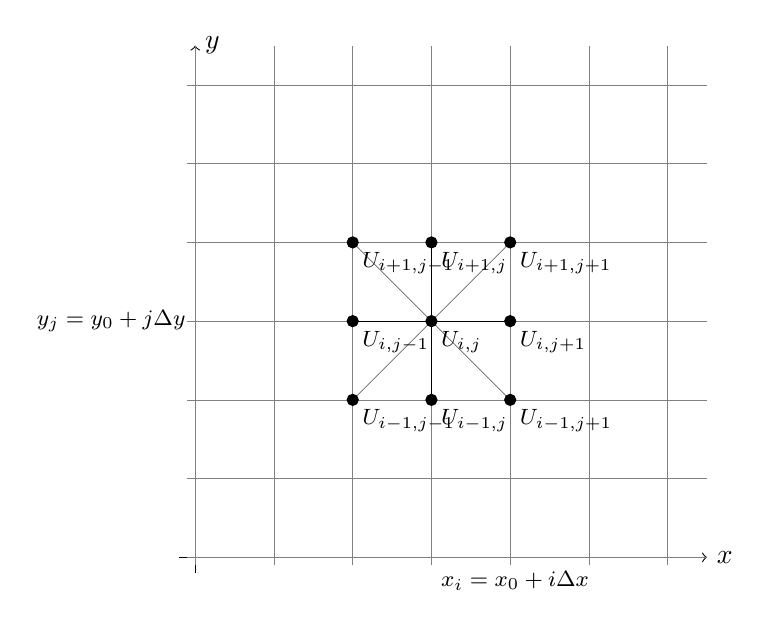
\begin{tikzpicture}
    \draw [->](0,-0.2)--(0,6.5) node[right]{$y$};
    \draw [->](-0.2,0)--(6.5,0) node[right]{$x$};
    \foreach \i in {0,...,6} {
        \draw [very thin,gray] (\i, -0.1) -- (\i,6 + 0.5);
    }
    \foreach \i in {0,...,6} {
        \draw [very thin,gray] (-0.1,\i) -- (6 + 0.5,\i);
    }
    
    \draw (3,-0.3) node[right]{\footnotesize{$x_i = x_0 + i\Delta x$}};
    \draw (0, 3) node[left]{\footnotesize{$y_j = y_0 + j\Delta y$}};
    
    \filldraw[black] (3, 3) circle (2pt) node[anchor=north west] {\footnotesize{$U_{i, j}$}};
    \filldraw[black] (2, 3) circle (2pt) node[anchor=north west] {\footnotesize{$U_{i, j-1}$}};
    \filldraw[black] (4, 3) circle (2pt) node[anchor=north west] {\footnotesize{$U_{i, j+1}$}};
    \filldraw[black] (3, 2) circle (2pt) node[anchor=north west] {\footnotesize{$U_{i-1, j}$}};
    \filldraw[black] (3, 4) circle (2pt) node[anchor=north west] {\footnotesize{$U_{i+1, j}$}};
    \filldraw[black] (4, 4) circle (2pt) node[anchor=north west] {\footnotesize{$U_{i+1, j+1}$}};
    \filldraw[black] (2, 2) circle (2pt) node[anchor=north west] {\footnotesize{$U_{i-1, j-1}$}};
    \filldraw[black] (4, 2) circle (2pt) node[anchor=north west] {\footnotesize{$U_{i-1, j+1}$}};
    \filldraw[black] (2, 4) circle (2pt) node[anchor=north west] {\footnotesize{$U_{i+1, j-1}$}};
    
    \draw [ultra thin] (3, 3) -- (2, 3);
    \draw [ultra thin] (3, 3) -- (4, 3);
    \draw [ultra thin] (3, 3) -- (3, 2);
    \draw [ultra thin] (3, 3) -- (3, 4);
    \draw [ultra thin] (3, 3) -- (4, 4);
    \draw [ultra thin] (3, 3) -- (2, 2);
    \draw [ultra thin] (3, 3) -- (4, 2);
    \draw [ultra thin] (3, 3) -- (2, 4);
    
\end{tikzpicture}
    \caption{Caption}
    \label{fig:stencil+grid}
\end{figure}



\clearpage